%!TEX root = main.tex

\section{Analysis of Voice Recognition}

\begin{figure}[th]
\centering
	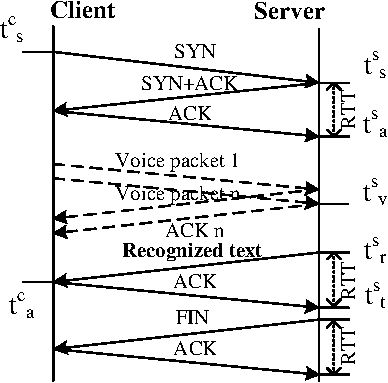
\includegraphics[scale=0.7]{voice_estimate_rtt}
\caption{Time-line in voice recognition flow.}
\label{fig:voice_estimate_rtt}
\end{figure}

Voice recognition consists of mobile terminals uploading the voice data and server returning back the recognized query text. Figure~\ref{fig:voice_estimate_rtt} shows the typical time-line of a voice recognition flow. The following web search is initialized by mobile clients once they receive the recognized text at $t^c_a$. That said, the finish time of a recognition flow measures the duration from $t^c_s$ to $t^c_a$. But we do not have these two timestamps from server side where we collected our datasets. Alternatively, we approximate the finish time with $T_s=t^s_t - t^s_s$. This finish time however includes the time consumed by servers automatically translating speech to text ($T_r=t^s_r - t^s_v$), which is not relevant to network performance\footnote{The time duration needed for translating voice to text is dependent on the used speech recognition technologies and we are not allowed by Qihoo to contain this statistic.} and out of our interests in this paper. We thus redefine the finish time as $T_s-T_r$.

\begin{figure}[th]
	\centering
	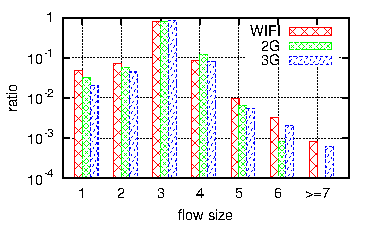
\includegraphics[width=0.8\linewidth]{voice_flow_size}
	\caption{The number of voice data packets in voice recognition flows.}
	\label{fig:voice_flow_size}
\end{figure}

We can observe from Figure~\ref{fig:voice_estimate_rtt} that the finish time can be approximated by $2\times RTT$ plus the time duration for the the voice data uploading if no packet loss happens. We measure the number of voice data packets in all flows in Figure~\ref{fig:voice_flow_size} for the three major access types, where $y$-axis is in log scale. Independent of the access type, 80\% of voice recognition flows contains no more 3 voice data packets and nearly all flows contain no more than 7 data packets. Given that the initial congestion window in current Android TCP/IP stack is set to 10 segments\cite{dukkipati2010argument}, the voice data could be transmitted in the initial congestion window. However, since any packets (including SYN) might be delayed, disordered or dropped by network, the finish time might vary greatly. In what follows, we will look at each TCP performance factor and its impact on flow finish time. 


\subsection{Impact of RTT}

As illustrated in Figure~\ref{fig:voice_estimate_rtt}, we can measure at most 3 RTTs from the server side in a voice recognition flow. However, RTT is ambiguous when the corresponding segments for RTT measures are retransmitted. To tackle this problem, we use the following methodology to determine the minimal RTT. If there is no retransmission of SYN packet, $t^s_a - t^s_s$ is used as the RTT of the flow, i.e. the RTT is measured during 3WHS. Otherwise, the RTT measured during connection termination is preferred if the FIN packet is not retransmitted. In the case that both of the above RTTs are ambiguous, $t^s_t - t^s_r$ is used as the measured RTT. We have verified using our datasets that $t^s_a - t^s_s$ is the minimal RTT in more than 60\% of flows, and is less than 2 times of the minimal RTT in 95\% of flows. Thus it is reasonable to assume that the RTT measured using the above methodology is close to the minimal RTT of the flow.

\begin{figure}[th]
\centering
	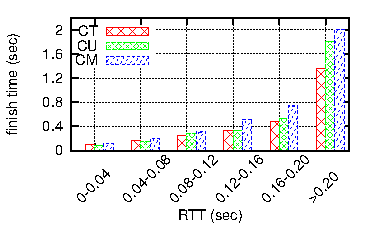
\includegraphics[width=0.8\linewidth]{voice_rtt}
\caption{Distribution for RTT of voice recognition flows.}
\label{fig:voice_rtt}
\end{figure}

Figure~\ref{fig:voice_rtt} plots the distribution for measured RTT of individual voice recognition flows. 2G and 3G flows experience similar RTT with a median around 0.03 second. WiFi flows on the other hand exhibit a higher RTT with a median around 0.05. In particular, while 95\% of 2G/3G flows have a RTT less than 0.1 second, as many as 20\% of WiFi flows have a RTT larger than this value. 

\begin{figure}[th]
\centering
	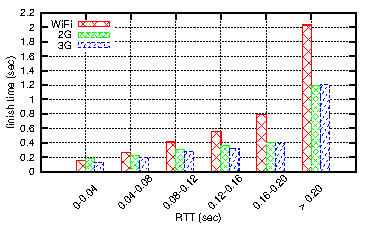
\includegraphics[width=0.8\linewidth]{voice_rtt_finish_time}
\caption{Impact of RTT on finish time.}
\label{fig:v_rtt_time}
\end{figure}

RTT is a major factor that affects TCP performance. We further examine the impact of RTT on flow finish time in Figure \ref{fig:v_rtt_time}. We observe that for flows with RTT no larger than 0.2 second, the finish time increases in proportional to the RTT: the ratio of finish time to RTT is about 2.5 for 2G/3G flows and about 4 for WiFi flows. As we explained in Figure \ref{fig:voice_estimate_rtt}, the finish time is approximately $2RTT$ plus the time for voice data uploading. Thus, the difference of the ratio between cellular network and WiFi network comes from the time for data uploading. One possibility is that the RTT during data transferring in WiFi network is significantly larger than the RTT measured during connection establishment (i.e. 3WHS) \cite{UM-CS-2012-022}, where we obtained most of the RTTs. It seems that 2G and 3G networks provide similar performance in terms of RTT during 3WHS and data transferring. 

The finish time becomes extremely large when RTT is beyond 0.2 second. Such a large RTT is an indication of network congestion as in TCP Vegas\cite{brakmo1995tcp} and FastTCP\cite{wei2006fast}. In other words, it is likely that the flow is traversing congested network and may encounter packet loss, which takes a relatively long time for recovery.

\subsection{Impact of packet disordering}
\label{sec:v_pd}


\begin{figure*}[th]
\centering
	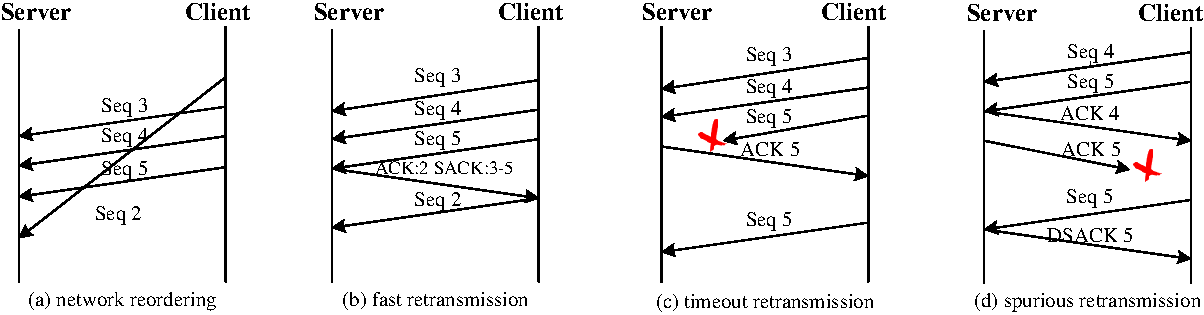
\includegraphics[scale=0.7]{voice_flow_estimate_retrans}
\caption{Server could not distinguish packet reordering events, which are (a) network reordering, (b) fast retransmit, and (c) timeout retransmission. Server may identify some timeout retransmissions as long packet delay (d).}
\label{fig:voice_flow_estimate_retrans}
\end{figure*}

Another factor that could heavily impact the finish time is the network congestion events, which include packet loss, fast retransmit, packet delay and packet reordering. However, as a TCP receiver, server could not identify the exact network congestion event. For example, server observe the same packet sequence number for Figure~\ref{fig:voice_flow_estimate_retrans}(a), \ref{fig:voice_flow_estimate_retrans}(b) and \ref{fig:voice_flow_estimate_retrans}(c), despite that they depict 3 types of congestion: packet reordering in Figure~\ref{fig:voice_flow_estimate_retrans}(a), fast retransmit in Figure~\ref{fig:voice_flow_estimate_retrans}(b) and timeout retransmission in Figure~\ref{fig:voice_flow_estimate_retrans}(c). Moreover, the server is also not able to identify whether the packet is a retransmitted packet or a delayed packet in \ref{fig:voice_flow_estimate_retrans}(d). These observations show the hardness of performing TCP analysis at server side for uploading sessions. 

% accurately identify the congestion event in Figure~\ref{fig:voice_flow_estimate_retrans}(d) is a timeout retransmission, the client retransmits the segment 5 when RTO timer is triggered, which could be caused by either the previous sent segment 5 is lost or delayed. Server in this case could not detect whether the packet is a retransmitted packet or a delayed packet. In fact, server can only detect unnecessary retransmission when receiving the same data packet twice, and notifies the spurious retransmission to client via Duplicate SACK~\cite{rfc3078} as shown in Figure~\ref{fig:voice_flow_estimate_retrans}(d). 

We thus directly use the number of disordered packets, a metric that server can accurately obtained, to capture the network congestion characteristics. In the example shown in Figure~\ref{fig:voice_flow_estimate_retrans}(a), the number of disordered packets is 1. As we show in Figure~\ref{fig:voice_flow_estimate_retrans}, a disordered packet seen by the serve could be caused by either packet reordering, fast retransmit or timeout retransmission. We show the distribution for the number of disordered packets in Table~\ref{tab:voice_reorder}.

\begin{table}[th]
\caption{Distribution for the number of disordered packets.}
\label{tab:voice_reorder}
\centering
\renewcommand{\arraystretch}{1.1}
\begin{tabular}{c|c|c|c}
\toprule
\# disord. pkts & WiFi & 2G & 3G \\
\hline
0 & 96.7\% & 94.4\% & 93.3\% \\
%\hline
1 & 3.03\% & 5.5\% & 6.6\% \\
%\hline
%2 & 0.1\% & - & - \\
%\hline
$\ge$2 & 0.2\% & - & - \\
\bottomrule
\end{tabular}
\end{table}

As expected, the majority of flows experience no packet disordering. But we did observe that more than 5\% of 2G/3G flows and 3\% of WiFi flows have one disordered packet. The fraction of flows having more than 2 disordered flows is negligible. Given that in most cases, the voice data only consists of 3 packets, even one disordered packet could severely degrade the uploading performance as shown in Figure \ref{fig:voice_reorder}.


\begin{figure}[th]
\centering
	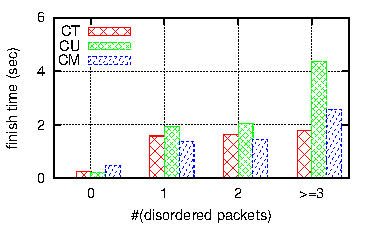
\includegraphics[width=0.8\linewidth]{voice_reorder}
\caption{Impact of packet disordering on finish time.}
\label{fig:voice_reorder}
\end{figure}

We can see from Figure \ref{fig:voice_reorder} that one disordered packet in 2G/3G uploading flows could increase the median finish time from 10 ms to 60 ms, while for WiFi flows we even observe as many as 20\% of those suffering from packet disordering cannot finish the uploading within 1 second. When receiving a disordered packet, server feeds back to the client with SACK (as shown in Figure~\ref{fig:voice_flow_estimate_retrans}(b)). Client will retransmit the packet in the hole (\ie the disordered packet) after collecting 3 SACKs. In the case that not sufficient number of SACKs can be collected, client has to rely on timeout retransmission for a RTO, which can be several times or tens of RTT. That said, the increased finish time might be caused by either packet delay, fast retransmit or timeout retransmission as stated in Figure~\ref{fig:voice_flow_estimate_retrans}. Unfortunately, we cannot identify how much each of these congestion events contributes using the datasets collected from server side.

The significance of the impact of packet disordering on finish time is also dependent on RTT, because both the waiting time for fast retransmit and timeout retransmission timer (i.e. RTO) depend on the RTT. To further assess the objective impact of packet reordering by excluding the possible effect of other covariates (like RTT), we implement a non-parametric factorial analysis framework using a Quasi Experimental Design (QED) \cite{krishnan2013video}. In QED, each uniformly sampled individual $u$ is compared with an individual $v$ randomly selected from those that have identical covariates with $u$ but the cause variable (packet reordering in our context). And thus, any outcome difference between these two individuals can be attributed to the cause variable we are tracking. 

In detail, we bin the voice recognition flows of each access type into two groups: those with no disordered packet ($G_1$) and those with 1 disordered packet ($G_2$). For each flow $u \in G_1$, we randomly choose a flow $v$ from $G_2$ that has similar RTT (i.e. the difference is less than 40 ms) and and the same condition whether encountering a timeout retransmission that is identified by the methodology in Section \ref{sec:v_rto}. We record the outcome difference as $o_{u,v} = (finish\_time_{v} - finish\_time_{u}) / finish\_time_{u})$. Finally, we average all the outcome differences over the matched pairs and use this average difference to gauge the impact of packet disordering.

\begin{table}[th]
\caption{QED results for the impact of packet disordering.}
\label{tab:voice_qed_reorder}
\centering
\renewcommand{\arraystretch}{1.1}
\begin{tabular}{c|c|c|c}
	\toprule
	 & WiFi & 2G & 3G \\
	\midrule
	QED & 6.42 & 3.37 & 4.45 \\
	\bottomrule
\end{tabular}
\end{table}

Table~\ref{tab:voice_qed_reorder} presents the QED results, which show that only one disordered packet can lead to an increase of finish time by $3-6$ times. The larger finish time increase of WiFi flows than 2G/3G flows is possibly because the packet disordering events observed by servers for WiFi flows are more likely to be timeout retransmission. The observations imply that the performance of short TCP flows for uploading is very sensitive to the network characteristics. 

\subsection{Impact of timeout retransmission}\label{sec:v_rto}

\begin{figure}[th]
\centering
	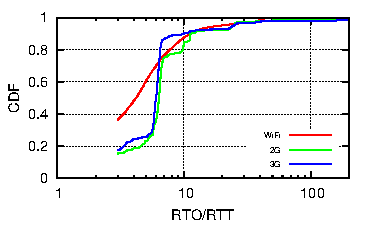
\includegraphics[width=0.8\linewidth]{voice_rtt_rto_ratio}
\caption{Distribution of RTO/RTT}
\label{fig:rto_rtt}
\end{figure}

Timeout retransmission indicates a severe network congestion that would takes a RTO for recovery. As we have shown in Figure  \ref{fig:voice_flow_estimate_retrans}, the server is unable to directly identify a timeout retransmission. We thus rely on the time gap between actual arrival time and the estimated arrival time of individual packets to detect timeout retransmissions, where the estimated arrival time is calculated according to that of preceding and subsequent packets. For example, given receiving data packets $s_1, s_3, s_2$, the estimated arrival time of $s_2$ is the mean value of the arrival time of $s_1$ and $s_3$. In the case that this gap is even larger than RTO, the transmission of the packet is identified as a timeout retransmission. However, the server does not know the client-side RTO. We thus have to estimate the RTO. RTO in TCP implementation is set to $\text{SRTT} + max(200ms, 4 \text{ RTTVAR})$\cite{rfc62982011computing}, where SRTT is close to RTT, and RTTVAR is approximately $RTT/2$, i.e. $\widehat{RTO} \approx RTT + max(200ms, 2 RTT)$. It is noteworthy that the timeout retransmissions identified using the above methodology show the same behavior as that illustrated in Figure \ref{fig:voice_flow_estimate_retrans}(d). As such, they are not overlapped with the those shown in Figure \ref{fig:voice_flow_estimate_retrans}(d), which are identified as packet disordering flows in Section \ref{sec:v_pd}.

Figure \ref{fig:rto_rtt} plots the distribution of RTO/RTT. We can observe the RTO is around several time of RTT, but can be as large as 20$-$30 times of RTT. As a time retransmission takes a RTO for recovery, our observation reveals the extremely large impact of timeout retransmission that could have on flow finish time.

\begin{table}[th]
\centering
\renewcommand{\arraystretch}{1.1}
\caption{Flows with timeout retransmission.}
\label{tab:voice_stats}
\begin{tabular}{l|c|c|c}
	\toprule
	 & WiFi & 2G & 3G \\
	\midrule
	% packet reordering & 3.2\% & 5.6\% & 6.2\% \\
	% \hline
	3WHS retx & 2.6\% & 1.4\% & 0.8\% \\
	\hline
	data retx & 9.5\% & 8.0\% & 7.3\% \\
	% \hline
	% incomplete transmission & 0.2\% & 0.3\% & 2.4\% \\
	\bottomrule
\end{tabular}
\end{table}

Table~\ref{tab:voice_stats} lists the percentage of flows that suffer from at least one timeout retransmission. The timeout retransmission could happen either during 3-way handshake (3WHS) or in data transmission. While the timeout retransmission during 3WHS is less likely to happen compared with timeout retransmission during data uploading, its impact might be even larger. This is because the initial RTO is set to 1 second \cite{rfc62982011computing} as there is no RTT measured. This RTO value is often much larger than that computed during data uploading. Users might quit the app during this the time period for recovery. 

Regardless of the access type, we observe as many as over 7\% of the voice data uploading flows suffer from at least one timeout retransmission. Such a large fraction of timeout retransmission flows can be explained by the fact that almost all the voice recognition flows contain no more than 6 voice data packets. When one of the last three packets is dropped, the sender (i.e. client) has to rely on RTO for retransmission. This behavior is similar to the tail lost one identified in \cite{flach2013reducing}. But in the voice data uploading context, the server is no longer a sender and thus unable to eliminate such kind of RTO retransmissions by gently send redundant packets as proposed in \cite{flach2013reducing}. Our results highlight the necessary of TCP optimization for uploading from server side. 

\begin{figure}[th]
\centering
	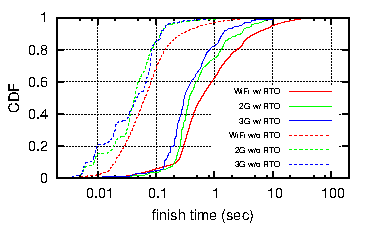
\includegraphics[width=0.8\linewidth]{voice_timeout}
\caption{CDF of finish time of flows with and without RTO.}
\label{fig:voice_rto}
\end{figure}

We finally compare the finish time between flows with and without timeout retransmission in Figure~\ref{fig:voice_rto}, where the x-axis is in log scale. The timeout retransmission increases the median finish time from 64 ms to 595 ms. This is not surprising given that RTO is several times of the RTT. In fact, since the number of voice data packets is relatively small ($\le 6$), which can be updated within $2\times RTTs$, the time retransmission time (i.e. RTO) will dominate the finish time of those flows that experience timeout retransmissions.  Overall, a larger fraction of WiFi flows suffer from timeout retransmission compared with 2G/3G flows, which partially explains the larger finish time observed in Figure \ref{fig:voice_finish_time}.

\subsection{Summary of Voice Recognition Analysis}

The key observations on voice recognition flows are summarized as follows.
\begin{itemize}
	\item Almost all voice recognition flows contain less than 7 data packets, which could be fitted into the initial congestion window from Android client. Thus ideally the voice data could be transmitted in 1 RTT.
	\item Finish time is affected by RTT. For flows with smaller RTT (less than 200ms in WiFi), the finish time is proportional to the RTT value. However, flows with larger RTT experience intolerably long finish time, caused by timeout retransmission.
	\item Flows in WiFi network experience 2-3 times longer finish time than those in cellular network, because of larger RTT.
	\item About 10\% of flows experience timeout retransmission when transmitting data, which make the finish time one order of magnitude larger than those without timeout retransmission.
	\item A non-negligible fraction of flows (0.8\%-2.6\%) experience retransmission when establishing connections, which has similar impact like RTO in data transfer.
\end{itemize}
